\newpage
\section{Week 8}
\subsection{Derivation}
We have following equations
\begin{eqnarray}
	\partial_z F(z\bar{z}) = \bar{z}F'(z\bar{z})\\
	\partial_{\bar{z}} F(z\bar{z})= zF'(z\bar{z})
\end{eqnarray}
Combining the definition of $\dot{F}$, we have
\begin{equation}
	\dot{F} = z \partial_z F(z\bar{z}) = \bar{z} \partial_{\bar{z}} F(z\bar{z})
\end{equation}
Since $F(z\bar{z})= z^4 \langle T(z,\bar{z}) T(0,0) \rangle$, we have 
\begin{equation}
	\dot{F} = \bar{z} \partial_{\bar{z}} \big(z^4 \langle T(z,\bar{z}) T(0,0)\rangle \big) = z^4\bar{z} \langle \partial_{\bar{z}}T(z,\bar{z})T(0,0) \rangle
\end{equation}
Similarly, for $G$, we have
\begin{equation}
	\begin{split}
	\frac{1}{4} \dot{G} &= \frac{1}{4}\big(z \partial_z G(z\bar{z})\big)\\
	&=\frac{1}{4} \big(z\partial_z (z^3\bar{z}\langle \Theta(z,\bar{z})T(0,0) \rangle ) \big)\\
	&= \frac{3}{4} z^3 \bar{z}\langle \Theta(z,\bar{z}) T(0,0) \rangle + \frac{1}{4} z^4 \bar{z} \langle \partial_z \Theta(z,\bar{z}) T(0,0) \rangle \\
	&= \frac{3}{4}G - z^4 \bar{z} \langle \partial_{\bar{z}} T(z,\bar{z})T(0,0) \rangle \\
	&= \frac{3}{4} G -\dot{F}
	\end{split}
\end{equation}
With the relation $\frac{1}{4} \langle\partial_z \Theta(z,\bar{z}) T(0,0) \rangle = \langle T(z,\bar{z}) T(0,0) \rangle$, we get
\begin{equation}
\frac{1}{4} \dot{G} = \frac{3}{4} G -\dot{F}
\end{equation}
It implies $\dot{F} + \frac{1}{4} \dot{G} - \frac{3}{4} G=0$. Furthermore, we have
\begin{equation}
\label{eq10}
	\begin{split}
	\dot{G} & = \bar{z} \partial_{\bar{z}} \big(z^3 \bar{z} \langle T(z,\bar{z}) \Theta(0,0) \rangle \big)\\
	& = z^3 \bar{z} \langle T(z,\bar{z}) \Theta(0,0) \rangle + z^3 \bar{z}^2 \langle \partial_{\bar{z}} T(z,\bar{z}) \Theta(0,0) \rangle \\
	&= G - \frac{1}{4} z^3 \bar{z}^2 \langle \partial_z \Theta(z,\bar{z})\Theta(0,0)\rangle
	\end{split}
\end{equation}
and for $H$, we have
\begin{equation}
\label{eq11}
	\begin{split}
	\dot{H} & = z \partial_z \big( z^2 \bar{z}^2 \langle \Theta(z,\bar{z}) \Theta(0,0) \rangle \big)\\
	& =z \big(2 z \bar{z}^2 \langle \Theta (z,\bar{z}) \Theta(0,0) \rangle + z^2 \bar{z}^2 \langle \partial_z \Theta(z,\bar{z}) \Theta(0,0) \rangle \big)\\
	& = 2H + z^3 \bar{z}^2 \langle \partial_z \Theta(z,\bar{z}) \Theta(0,0)\rangle 
	\end{split}
\end{equation}
Combining equation \ref{eq10} and \ref{eq11}, we get 
\[
\dot{G} - G + \frac{1}{4} \dot{H} - \frac{1}{2} H =0
\]
%%%%
By computation, we have
\begin{equation}
	\frac{\partial}{\partial R} C(z\bar{z},g) = C'(z \bar{z},g) 2R
\end{equation}
It implies that 
\begin{equation}
	\begin{split}
	R \frac{\partial}{\partial R} C(z\bar{z},g) &= 2R^2 C'(z\bar{z})\\
	 &= 2z \bar{z}C'(z\bar{z},g) \\
	 &= 2 \dot{C} = -\frac{3}{2}H
	\end{split}
\end{equation}
When $R=1$, we have 
\[
R \frac{\partial}{\partial R} C(z\bar{z},g)= - \frac{3}{2} \beta^a(g)\beta^b(g) \langle \mathcal{O}_a(x) \mathcal{O}_b(x) \rangle 
\]
since $\Theta(x)= \beta^a(g) \mathcal{O}_a(x)$. Hence we get
\begin{equation}
	\beta^a \frac{\partial}{\partial g^a} C(g)= -\beta^a(g)\beta^b(g) \langle \mathcal{O}_a(x) \mathcal{O}_b(x) \rangle 
\end{equation}
%%%
\subsection{\beta-functions}
To compute the integral 
\[
\int_{a < |x_{12}| < a(1+\delta \lambda)} \langle \mathcal{O}(x_1) \mathcal{O}(x_2) \rangle \frac{d x_1}{a^{2-h}} \frac{d x_2}{a^{2-h}}
\]
With OPE $\mathcal{O}(x_1)$ and $\mathcal{O}(x_2)$, we have 
\begin{equation}
	\langle \mathcal{O}(x_1) \mathcal{O}(x_2) \rangle = \frac{C}{|x_{12}|^h} \langle\mathcal{O}(x_2)\rangle
\end{equation} 
Hence we have
\begin{equation}
\label{eq13}
	\begin{split}
	\int_{a < |x_{12} | < a(1+\delta\lambda)} \langle \mathcal{O}(x_1) \mathcal{O}(x_2) \rangle \frac{d x_1}{a^{2-h}} \frac{d x_2}{a^{2-h}} &= \int_{a < |x_{12} | < a(1+\delta\lambda)} \frac{C}{|x_{12}|^h} \frac{dx_1}{a^{2-h}} \langle \mathcal{O}(x_2) \rangle  \frac{dx_2}{a^{2-h}}\\
	&
	\end{split}
\end{equation}
Since $|x_{12}| \sim a$ as $\delta$ infinitesimal, \ref{eq13} becomes 
\begin{equation}
	\begin{split}
	\int_{a < |x_{12} | < a(1+\delta\lambda)} \langle \mathcal{O}(x_1) \mathcal{O}(x_2) \rangle \frac{d x_1}{a^{2-h}} \frac{d x_2}{a^{2-h}} & = a^{-2}C \int_{a < |x_{12} | < a(1+\delta\lambda)} dx_1 \int \langle \mathcal{O}(x) \rangle \frac{dx}{a^{2-h}}\\
	\end{split}
\end{equation}
Since the area of $a < |x_{12} | < a(1+\delta\lambda $ is $\delta \lambda \pi a^2 (\delta \lambda +2)$, we have
\begin{equation}
	\begin{split}
	\int_{a < |x_{12} | < a(1+\delta\lambda)} \langle \mathcal{O}(x_1) \mathcal{O}(x_2) \rangle \frac{d x_1}{a^{2-h}} \frac{d x_2}{a^{2-h}} & = C \delta \lambda \pi (\delta\lambda +2) \int \langle \mathcal{O}(x)\rangle \frac{dx}{a^{2-h}}\\
	& \sim 2 \delta \lambda \pi C \int \langle \mathcal{O}(x) \rangle \frac{dx}{a^{2-h}}
	\end{split}
\end{equation}
Hence the second term is 
\[
\delta \lambda \pi C \hat{g}^2  \int \langle \mathcal{O}(x) \rangle \frac{dx}{a^{2-h}}
\]
Therefore, we get deformation
\begin{equation}
	\text{Def}_{\hat{g}}(\lambda) = \hat{g} + \delta(2-h) \lambda \hat{g} - \delta \pi C \lambda \hat{g}^2 + O(\hat{g}^3)(\lambda)
\end{equation}
Now we have 
\begin{equation}
	\frac{d \hat{g}}{d\lambda} = (2-h) \hat{g} - \pi C \hat{g}^2 + O(\hat{g}^3)
\end{equation}
The $\beta$-function is 
\[
\beta(\hat{g}) = (2-h) \hat{g} - \pi C \hat{g}^2 + O(\hat{g}^3)
\]
Hence near $\hat{g}=0$, we have the picture of curve of $\beta$-function
\begin{figure}[h]
	\centering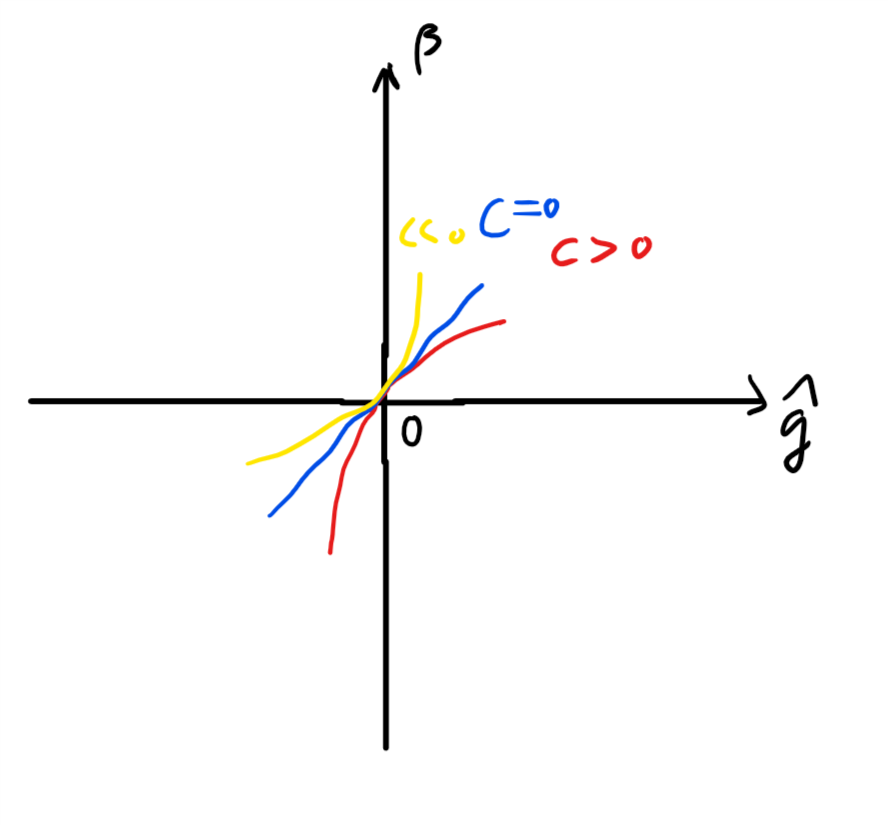
\includegraphics[scale=0.5]{PIC/hw8pic1.png}
\end{figure}
To solve equation
\begin{equation}
	\frac{d\hat{g}}{d\lambda} = - \pi C \hat{g}^2
\end{equation}
we separate variables
\[
- \frac{1}{\hat{g}^2} d \hat{g} = \pi C \lambda d\lambda
\]
Taking integrals of both sides, we get
\begin{equation}
\frac{1}{\hat{g}} = \pi C\lambda +K
\end{equation}
where $K$ is constant. When $\lambda=0$, $\hat{g} = g_*$, so $K = \frac{1}{g^*}$. Therefore,
\[
\hat{g}(\lambda) = \frac{g^*}{g^* \pi C \lambda +1}
\]
Since the $\beta$-function is
\[ 
\beta(\hat{g}) = - \pi C \hat{g}^2
\]
if $C < 0$, then $\beta > 0$, so $\mathcal{O}$ is marginal relevant. If $C=0$, then $\mathcal{O}$ is exactly marginal. If $C > 0$, then $\mathcal{O}$ is marginal irrelevant
